\subsection{Blockchain}
\label{sec:sota_blockchain}
    Eine Blockchain ist eine immer größer werdende Kette von Einträgen, die dezentral gespeichert wird. 
    Erstmals 2008 von Satoshi Nakamoto, ursprünglich als Peer-to-Peer Electronic Cash System ,,Bitcoin`` erfunden, fand die Technologie aufgrund ihren Vorteilen wie des dezentralen, anonymen Konzepts schnell viele <Anhänger>. \todo[color=cyan]{Einleitung schreiben}
    
    \subsubsection{Einführung in das Konzept}
    \label{sec:sota_blockchain_introduction}
    % Top-down Erklärung... Blockchain -> Block -> Transaktion -> Asset
    Bitcoin ist die erste digitale Währung, die ursprünglich ohne zentrale Autorität wie beispielsweise einer \gls{ttp} das bereits in \fref{sec:sota_doublespend} vorgestellte Double-Spending Problem lösen sollte\cite{Nakamoto2008}. 
    Übertragen auf Bitcoin bedeutet es, dass der Empfänger sichergehen können muss, dass die vorigen Besitzer keine vorherigen Transaktionen signiert hatte \cite{Nakamoto2008}\todo[color=yellow]{Übersetzung okay?}.
    Dies wird mittels kryptographischem Beweis anstatt des laut \citeauthor{Nakamoto2008} vorstellten mangelhaften Modells der \gls{ttp} gelöst\todo[color=orange]{besser ausdrücken}.
    Getätigte Transaktionen sollen nicht rückgängig machbar sein, in dem die Rückrechnung des Beweises rechnerisch zu aufwändig sein soll\cite{Nakamoto2008}.
    Somit wird der Verkäufer vor Täuschung geschützt und Treuhandmechanismen können einfach implementiert werden\cite{Nakamoto2008}.  
    
    Das Konzept \citeauthor{Nakamoto2008}s ermöglichte es somit zwei Entitäten, die sich gegenseitig nicht vertrauen müssen eine direkte Transaktion durchzuführen.
    Es müssen also alle Teilnehmer in einem Bitcoin-Netzwerk alle Transaktionen innerhalb des Netzwerkes kennen (Analog: Rollen des Ausstellers bzw. des Mint übernehmen)\todo[color=orange]{nachlesen}.
    Ebenso müssen alle Transaktionen für alle Teilnehmer einsehbar sein, also veröffentlicht werden.
    Weiterhin benötigt das System eine einzige Historie, in welcher alle vergangenen Transaktionen in der Reihenfolge ihres Auftretens stehen.
    Zuletzt benötigt der Empfänger des Coins einen Beweis, dass sich die Mehrheit der Konten zur Zeit der Transaktion einig waren, dass die aktuelle die erste entgegengenommene Transaktion des Coins ist. 
    \cite{Nakamoto2008}
    \todo[color=cyan]{timestamps?}
    \medskip\\
    
    \noindent Grundlegend ist die Blockchain eine verteilte Datenstruktur, die zwischen den Mitgliedern eines Netzwerkes repliziert und geteilt wird\cite{Christidis2016}.
    Die Knoten des Netzwerkes (genannt ,,Miner'`) fügen validierte, gegenseitig abgestimmte Transaktionen, die zu Blöcken gebündelt werden.
    Die Blockchain beinhaltet das maßgebliche ,,Hauptbuch'` von Transaktionen, welches im Endeffekt festlegt, wem was gehört.\todo[color=yellow]{meh}
    Dieses ,,Hauptbuch'` ist ein Log, dessen Einträge mit Zeitstempeln jeweils als Blöcke zusammengefasst werden.
    Das System ist so lange sicher, wie ,,ehrliche'` Knoten gemeinsam mehr Rechenleistung als eventuell zusammenarbeitende Angreifer haben\cite{Nakamoto2008}.
    
    \subsubsection{Transaktionen}
    \label{sec:sota_blockchain_trx}
	    Zunächst wurde mit digitalen Coins gehandelt, welche einer in Form einer Kette digitaler Signaturen modelliert wurden\cite{Nakamoto2008}.
	    In anderen Anwendungsbereichen außerhalb des Bereiches der Kryptowährungen wird von generalisierten Assets gesprochen.\todo[color=yellow]{richtig?}
	    \begin{figure}[H]
	    	\centering
	    	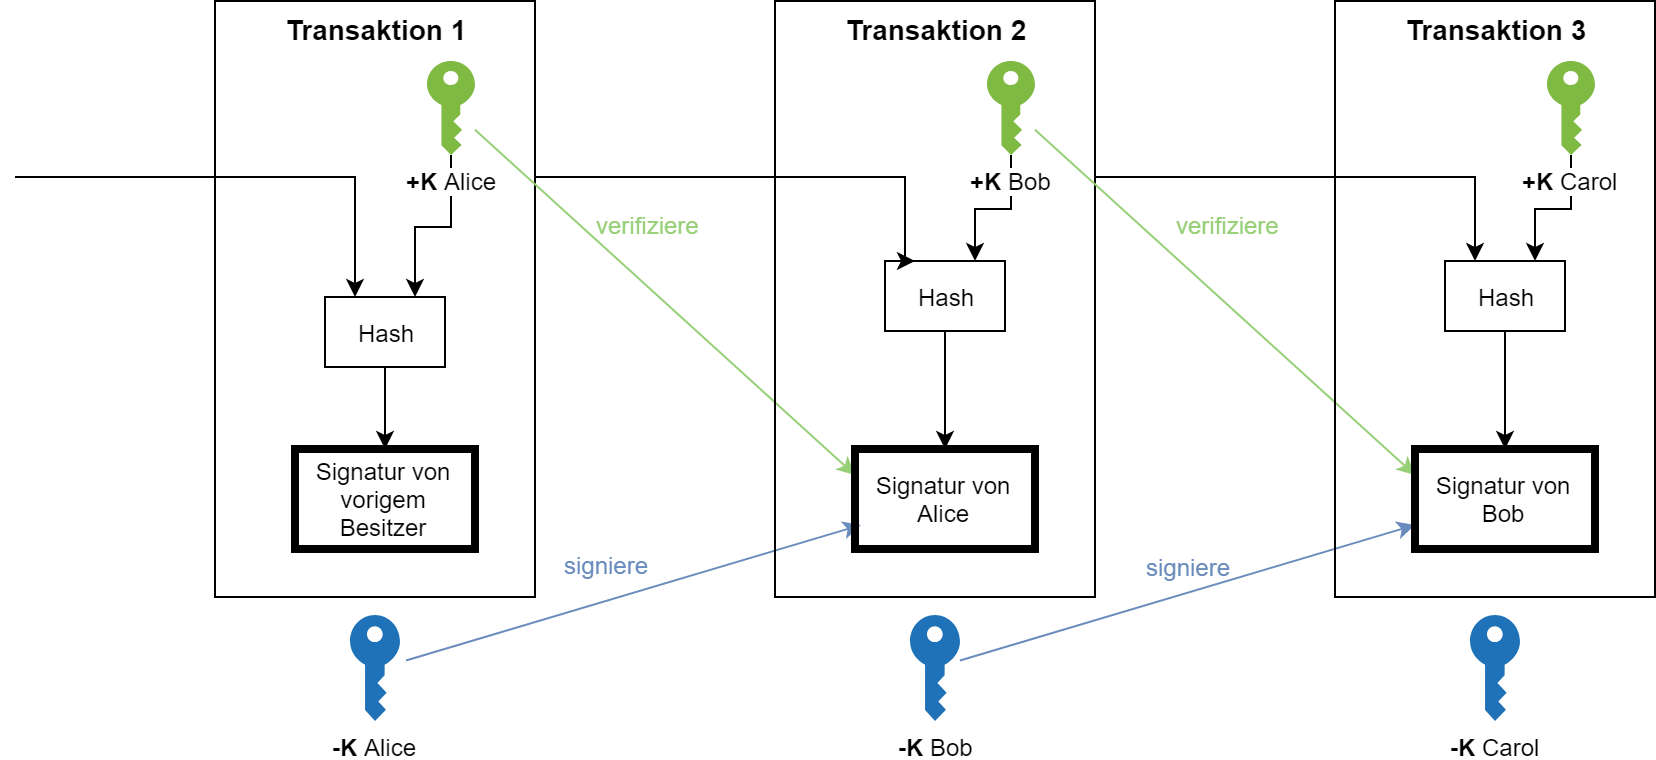
\includegraphics[width=0.9\textwidth]{graphics/transaction.png}
	    	\caption{Kette digitaler Signaturen}
	    	\label{fig:txio}
	    \end{figure}
    
	    Wie in \fref{fig:txio} dargestellt, werden Assets von einem Versender zu einem Empfänger transferiert, in dem der Sender einen Hash der vorigen Transaktion und den öffentlichen Schlüssel des Empfängers mit seinem eigenen privaten Schlüssel digital signiert und diese Hash dann am Ende des Assets anfügt.
	    Transaktionen können zudem mehrere Ein- und Ausgaben haben\cite{Nakamoto2008}.
	    Der Empfänger, sowie alle Teilnehmer des Netzwerkes können den Besitz des Assets über die Kette der digitalen Signaturen zurückverfolgen\cite{Nakamoto2008}.
    
    
    \begin{figure}[H]
        \missingfigure[figheight=4cm]{Bild mit Transaktion}
    \end{figure}
    
    \subsubsection{Sicherheit}
    \label{sec:sota_blockchain_security}
    Byzantine Fault Tolerance
    
    \subsubsection{Identity Management}
    \label{sec:sota_blockchain_identitymgmnt}
    \subsubsection{Self-Sovereign Identitity}
    \label{sec:sota_blockchain_sovreign}



